% !TeX spellcheck = en_US
%% 字体:方正静蕾简体
%%		 方正粗宋
\documentclass[a4paper,left=2.5cm,right=2.5cm]{article}

\usepackage[utf8]{inputenc}
\usepackage{fontspec}
\usepackage{cite}
\usepackage{xeCJK}
\usepackage{indentfirst}
\usepackage{titlesec}
\usepackage{longtable}
\usepackage{graphicx}
\usepackage{float}
\usepackage{rotating}
\usepackage{subfigure}
\usepackage{tabu}
\usepackage{amsmath}
\usepackage{setspace}
\usepackage{amsfonts}
\usepackage{appendix}
\usepackage{listings}
\usepackage{xcolor}
\usepackage{geometry}
\setcounter{secnumdepth}{4}
\titleformat*{\section}{\LARGE}
\renewcommand\refname{参考文献}
%\titleformat{\chapter}{\centering\bfseries\huge\wryh}{}{0.7em}{}{}
%\titleformat{\section}{\LARGE\bf}{\thesection}{1em}{}{}
\titleformat{\subsection}{\Large\bfseries}{\thesubsection}{1em}{}{}
\titleformat{\subsubsection}{\large\bfseries}{\thesubsubsection}{1em}{}{}
\renewcommand{\contentsname}{{\cjkfzcs \centerline{目{  } 录}}}
\setCJKfamilyfont{cjkhwxk}{华文行楷}
\setCJKfamilyfont{cjkfzcs}{方正粗宋简体}
\newcommand*{\cjkfzcs}{\CJKfamily{cjkfzcs}}
\newcommand*{\cjkhwxk}{\CJKfamily{cjkhwxk}}
\newfontfamily\wryh{Microsoft YaHei}
%\newfontfamily\ygyfryg{叶根友福荣银钩}
\newfontfamily\hwzs{华文中宋}
\newfontfamily\hwst{华文宋体}
\newfontfamily\hwfs{华文仿宋}
\newfontfamily\jljt{方正静蕾简体}
\newfontfamily\hwxk{华文行楷}
\newcommand{\verylarge}{\fontsize{60pt}{\baselineskip}\selectfont}  
\newcommand{\chuhao}{\fontsize{44.9pt}{\baselineskip}\selectfont}  
\newcommand{\xiaochu}{\fontsize{38.5pt}{\baselineskip}\selectfont}  
\newcommand{\yihao}{\fontsize{27.8pt}{\baselineskip}\selectfont}  
\newcommand{\xiaoyi}{\fontsize{25.7pt}{\baselineskip}\selectfont}  
\newcommand{\erhao}{\fontsize{23.5pt}{\baselineskip}\selectfont}  
\newcommand{\xiaoerhao}{\fontsize{19.3pt}{\baselineskip}\selectfont} 
\newcommand{\sihao}{\fontsize{14pt}{\baselineskip}\selectfont}      % 字号设置  
\newcommand{\xiaosihao}{\fontsize{12pt}{\baselineskip}\selectfont}  % 字号设置  
\newcommand{\wuhao}{\fontsize{10.5pt}{\baselineskip}\selectfont}    % 字号设置  
\newcommand{\xiaowuhao}{\fontsize{9pt}{\baselineskip}\selectfont}   % 字号设置  
\newcommand{\liuhao}{\fontsize{7.875pt}{\baselineskip}\selectfont}  % 字号设置  
\newcommand{\qihao}{\fontsize{5.25pt}{\baselineskip}\selectfont}    % 字号设置 

\usepackage{diagbox}
\usepackage{multirow}
\boldmath
\XeTeXlinebreaklocale "zh"
\XeTeXlinebreakskip = 0pt plus 1pt minus 0.1pt
\definecolor{cred}{rgb}{0.8,0.8,0.8}
\definecolor{cgreen}{rgb}{0,0.3,0}
\definecolor{cpurple}{rgb}{0.5,0,0.35}
\definecolor{cdocblue}{rgb}{0,0,0.3}
\definecolor{cdark}{rgb}{0.95,1.0,1.0}
\lstset{
	language=Matlab,
	numbers=left,
	numberstyle=\tiny\color{black},
	showspaces=false,
	showstringspaces=false,
	basicstyle={\footnotesize}\ttfamily,
	keywordstyle=\color{cdocblue}\bfseries,
	commentstyle=\color{cgreen},
	stringstyle=\color{cred},
	frame=lines,
	escapeinside=``,
	xleftmargin=1em,
	xrightmargin=1em, 
	%backgroundcolor=\color{cdark},
	aboveskip=1em,
	breaklines=true,
	tabsize=4
} 

\newfontfamily{\consolas}{Consolas}
\newfontfamily{\monaco}{Monaco}
\setmonofont[Mapping={}]{Consolas}	%英文引号之类的正常显示,相当于设置英文字体
\setsansfont{Consolas} %设置英文字体 Monaco, Consolas,  Fantasque Sans Mono
\setmainfont{Times New Roman}

\setCJKmainfont{华文中宋}

\newcommand*{\mytitle}
{
	
	\begingroup 
	\begin{center}
		\vspace*{0.05\paperheight} % White space at the top of the page
		\rule{\textwidth}{1.6pt}\vspace*{-\baselineskip}\vspace*{2pt} % Thick horizontal line
		\rule{\textwidth}{0.4pt}\\[\baselineskip] % Thin horizontal line
		{\yihao{\cjkhwxk {数学软件 \\[0.4\baselineskip]上机考试答题卷}}}\\[0.2\baselineskip] % Title
		\rule{\textwidth}{0.4pt}\vspace*{-\baselineskip}\vspace{3.2pt}		
		\rule{\textwidth}{1.6pt}\\[3\baselineskip]
		
\includegraphics[width=0.5\textwidth]{xiaohui.jpg}
		\vspace*{3\baselineskip} % Whitespace between 
		{\LARGE\hwzs
			\begin{longtable}{ll}
				\cjkfzcs{姓名:}& 汪利军\\
				\cjkfzcs{学号:}& 3140105707\\
				\cjkfzcs{班级:}& 统计1401\\
			\end{longtable}
		}\par
		\vspace*{1\baselineskip}
		{\Large\hwzs 2016.07.11}
	\end{center}
	\vfill
	\endgroup
}
\usepackage{lastpage}
\usepackage{fancyhdr}
\pagestyle{fancy}
\lhead{\space \qquad \space}
\chead{数学软件课程上机考试}
\rhead{\qquad\thepage/\pageref{LastPage}}
\begin{document}
	\begin{titlepage}
		\mytitle
	\end{titlepage}
	\begin{spacing}{1.6}
		
	\tableofcontents
	\end{spacing}
	\newpage
	\begin{spacing}{1.6}
		\section{参数}
		学号为$3140105707$,故$A=31401$,$B=05707=5707$
		于是有
		
		\begin{eqnarray}
		a &=& mod(A+B,13)=6\\
		B &=& mod(B,13)=0
		\end{eqnarray}
		\section{第一题}
		代入参数,方程为
		\begin{equation}
		x^3+7x+1=0
		\end{equation}
		\subsection{代码求解}
		下面是命令行窗口的运行命令及相应结果
	\begin{lstlisting}
	syms x
	>> syms x
	>> eqn = x^3+7*x+1 == 0;
	>> solx = solve(eqn,x)
	
	solx =
	
	root(z^3 + 7*z + 1, z, 1)
	root(z^3 + 7*z + 1, z, 2)
	root(z^3 + 7*z + 1, z, 3)
	
	>> x = (-10:0.001:10);
	>> y = x.^3+7*x+1;
	>> plot(x,y)
	>> S_vpa = vpa(solx)
	
	S_vpa =
	
	-0.14244425060428649657171963060493
	0.071222125302143248285859815302463 - 2.6486256385902599996106724277849i
	0.071222125302143248285859815302463 + 2.6486256385902599996106724277849i
	
	>> plot(x,y);
	>> hold on;
	>> line([-10,10],[0,0]);
	\end{lstlisting}
	\subsection{运行结果}
	该方程有一个实数根$x=-0.142444$,两个虚数根$x=0.071222\pm2.648625i$,
	图象如图(\ref{sol1})所示
	\begin{figure}[H]
		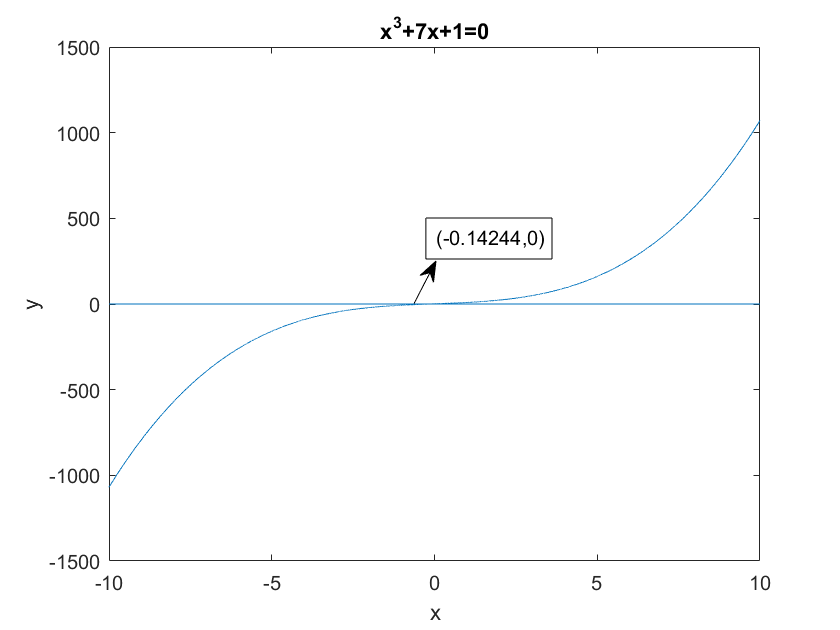
\includegraphics[width=0.9\textwidth]{image/result_1.png}
		\caption{第一题运行结果}
		\label{sol1}
	\end{figure}
	\section{第二题}
	代入参数,注意到第二个分段函数定义域为空,于是此时函数为
	\begin{equation}
	f(x)=\left\{
	\begin{array}{ll}
	cos(6*|x|)& 5\le x\le 6\\
	sin(6^x)& 6 < x\le 7
	\end{array}
	\right.
	\end{equation}
	\subsection{代码求解}
	注意此时$x2$不是从第一个元素开始取,故代码中有$x2=x2(2:end)$
	\begin{lstlisting}
	x1 = 5:0.001:6;
	x2 = 6:0.001:7;
	y1 = cos(6*abs(x1));
	x2 = x2(2:end);
	y2 = sin(6.^x2);
	plot(x1,y1,x2,y2);
	title('f(x)`函数图象`');
	xlabel('x');
	ylabel('y');
	\end{lstlisting}
	\subsection{运行结果}
	画出函数图像如图(\ref{sol2})所示
	\begin{figure}[H]
		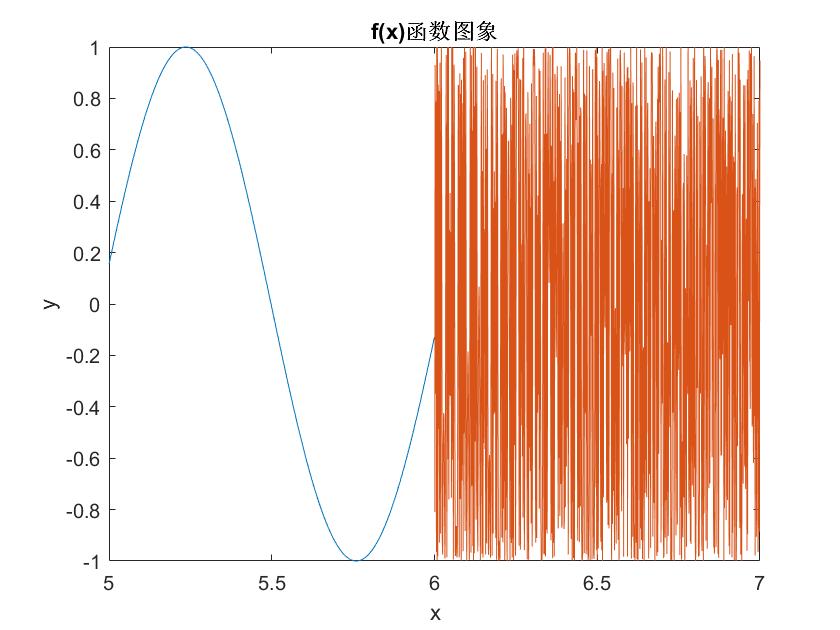
\includegraphics[width=0.8\textwidth]{image/result_2.png}
		\caption{第二题函数图像}
		\label{sol2}
	\end{figure}
	\section{第三题}
	代入参数$a=6,b=0$,则
	\begin{eqnarray}
	N &=& max(10*6,(6+4)*(0+2),(6+0)*(6+0))\\
	& =& max(60,20,36)\notag\\
	& = & 60\notag
	\end{eqnarray}
	\subsection{代码求解}
	\lstinputlisting{code/solve3.m}
	\subsection{运行结果}
	计算得到$sum=1830$,如图(\ref{sol3})所示
	\begin{figure}[H]
		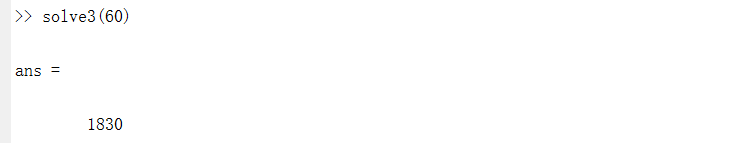
\includegraphics[width=0.8\textwidth]{image/result_3.png}
		\caption{第三题运行结果}
		\label{sol3}
	\end{figure}
	\section{第四题}
	代入参数$a=6,b=0$,于是需要绘制的图像为$\sqrt{x^2+6}+x$与$sin(x^2)$
	\subsection{代码求解}
	\lstinputlisting{code/solve4.m}
	\subsection{运行结果}
	生成函数图像如图(\ref{sol4})所示
	\begin{figure}[H]
		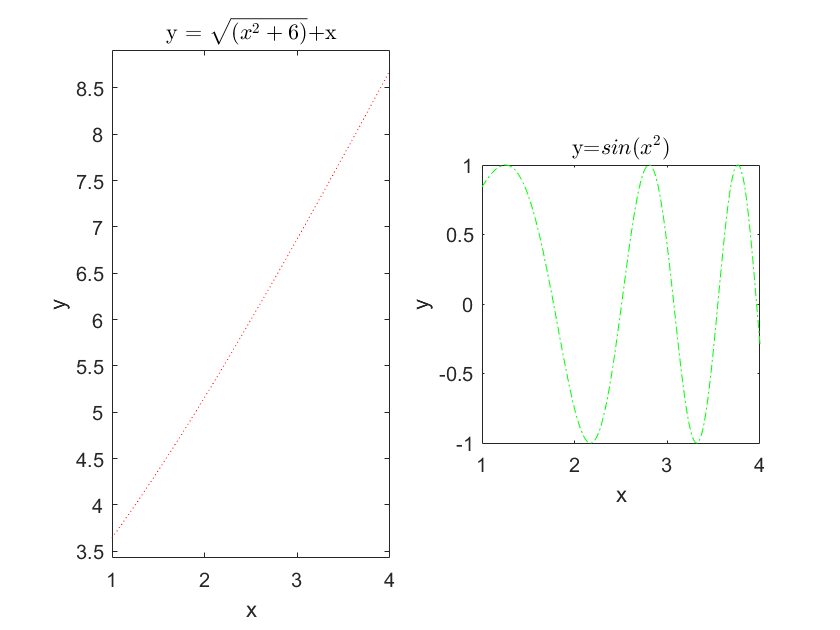
\includegraphics[width=0.8\textwidth]{image/result_4.png}
		\caption{第四题运行结果}
		\label{sol4}
	\end{figure}
	\section{第五题}
	代入参数$a=6,b=0$,则有
	\begin{equation}
	n = max(6+0,13-6,13-0) = 13
	\end{equation}
	\subsection{代码求解}
	编写solve5函数,输入$n$,返回矩阵$d$
	\lstinputlisting{code/solve5.m}
	\subsection{运行结果}
	运行结果如图(\ref{sol5})所示
	\begin{figure}[H]
		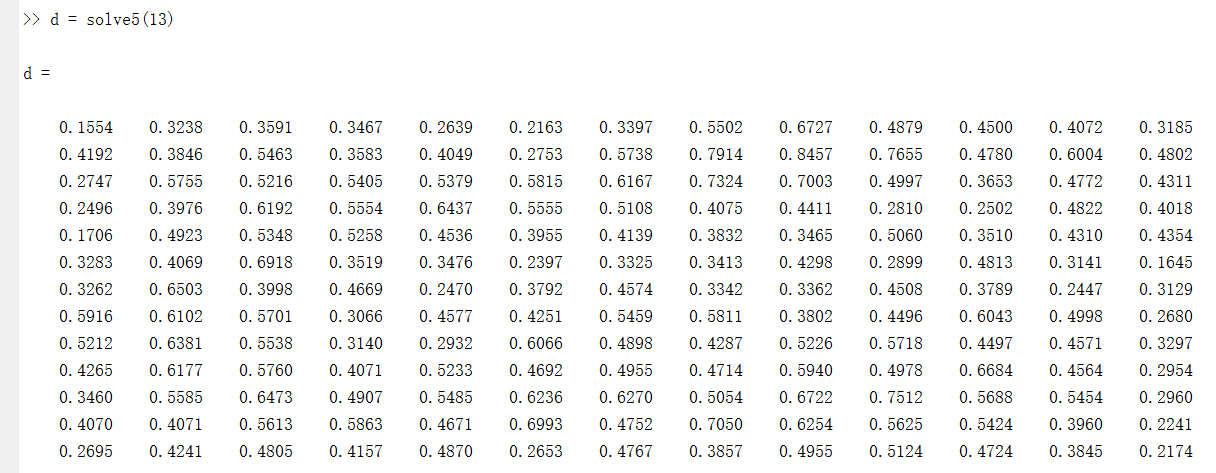
\includegraphics[width=0.8\textwidth]{image/result_5.png}
		\caption{第五题运算结果}
		\label{sol5}
	\end{figure}
	\end{spacing}
\end{document}
